En esta sección desarrollaremos y mostraremos los resultados de los experimentos para las siguientes
universidades:

\begin{itemize}
\item Universidad de Oxford(Reino Unido)
\item Universidad de Sydney (Australia)
\item Universidad de Ghana (Africa)
\end{itemize}

Para llevar adelante los experimentos utilizamos la herramienta descripta en la introducción. La cantidad de veces que ejecutamos nuestra versión de \texttt{traceroute} para cada universidad fue de \textbf{50}. Con esa cantidad lo que buscamos  es minimizar las oscilaciones en las rutas y tiempos fruto de balanceaos de carga de los routers.

Para identificar los saltos intercontinentales calculamos la variación en los \texttt{RTT} entre cada par de hops consecutivos, $\Delta RTT_{i}$, de la siguiente manera: \(\Delta RTT_{i} = \frac{RTT_{i} - RTT_{i-1}}{RTT_{i-1}}\), donde $2 \leq i \leq$ cantidad de hops. Siendo los candidatos a saltos intercontinentales los pares de hops con $\Delta RTT$ mayor al resto. A partir de este calculo, tendremos en cuenta la detección de falsos positivos y negativos contrastando nuestra inferencia con herramientas de geolocalización de direcciones IP, (\textbf{ref a geolookip o lo que sea}).

Por último, propondremos hipótesis para los casos de comportamiento anómalo.

\subsection{Universidad de Oxford}

Una vez mandados los paquetes y realizados los promedios, procederemos a graficar los tiempos resultantes.

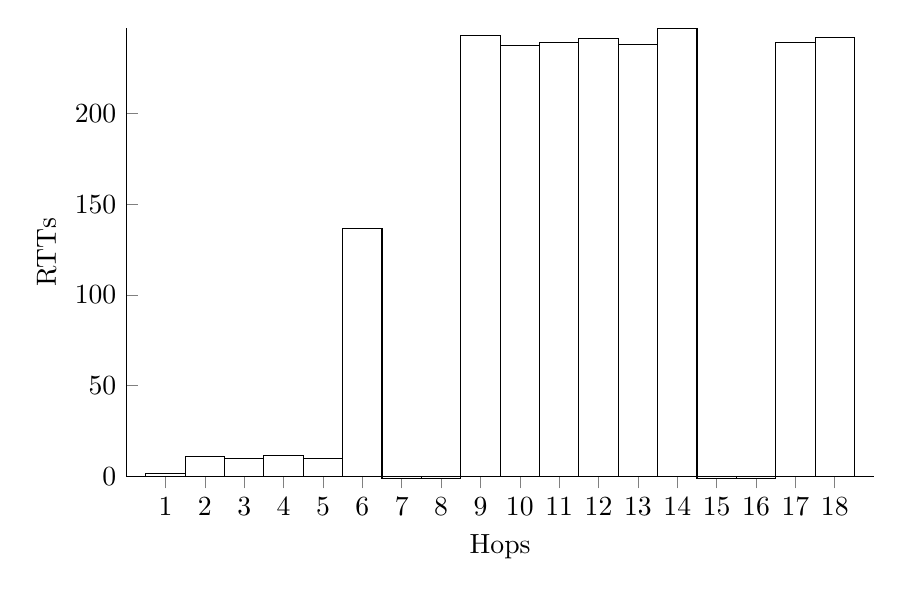
\begin{tikzpicture}
\begin{axis}[
    ybar,
    bar width=0.5cm, % Width of the bar
    x=0.5cm, % Distance between the centers of the bars
    enlarge x limits={abs=0.5cm}, % The distance between the center of the first bar and the left edge
    enlarge y limits=false,
    ymin=0,
    xtick=data,
    xlabel= {Hops},
    ylabel= {RTTs},
    symbolic x coords={1,2,3,4,5,6,7,8,9,10,11,12,13,14,15,16,17,18},
    point meta={y*100}, %y-Werte mal 100 für Prozent
    axis lines*=left,
    clip=false
    ]
\addplot [
    draw=black,
    fill=white,
    error bars/.cd,
        y dir=both,
        y explicit
    ] coordinates{(1,1.67)
        (2,10.90)
        (3,10.14)
        (4,11.67)
        (5,9.96)
        (6,136.57)
        (7,-1)
        (8,-1)
        (9,242.78)
        (10,237.21)
        (11,239.08)
        (12,241.48)
        (13,237.82)
        (14,246.91)
        (15,-1)
        (16,-1)
        (17,239.13)
        (18,241.63)};
\end{axis}
\end{tikzpicture}

Con este gráfico podemos claramente observar los saltos negativos y en los que no hubo respuesta(estos
últimos los notamos con RTT -1).

Cuando los tiempos de ida y vuelta reportados por traceroute son falsas ocurre la esta anomalía, conocida
como False Round-Trip Times . Generalmente hay dos razones, ya sean rutas de paquete asimétricos o enrutamiento
MPLS. Cuando los respectivos caminos hacia y desde el destino son asimétricos, es decir, los paquetes se
encaminan por senderos diferentes desde y hacia el objetivo, los tiempos de ida y vuelta pueden no
reflejar el tiempo real que tarda un paquete para llegar al destino. El ida y vuelta resultantes muestran
posteriormente los valores engañosos. La trayectoria real puede de hecho ser mucho más corto o más largo
que el tiempo de ida y vuelta indica, dependiendo de la situación.

MPLS es un caso similar al anterior y podría verse en que los tiempos de ida y vuelta casi equivalentes
para varios saltos en el resultado de traceroute.

Daremos nuestras hipótesis sobre que casos son los que identificamos.

\begin{itemize}
\item Entre 2 y 3. Claramente es paquetes asimétricos.
\item Entre 4 y 5. Consideramos que también es asimétricos. Aunque podría ser MLPS ya que en 3 tenemos un
RTT muy similar a 4.
\item Entre 9 y 10. Asimétrico.
\item Entre 12 y 13.Asimétrico.
%Tengo que identificar a 14 y 17.
\end{itemize}



Por otro lado tenemos los que no tuvieron respuesta. Esta es la anomalía es conocida como Missing Hops.
Se produce en general cuando un router está protegido por un firewall o de configurado otro modo para no
generar errores excesivos ICMP TTL. En nuestro caso tenemos 7, 8, 15, 16.

El hops 6 pertenece a Kansas, Estados Unidos pero el 9 pertenece a Reino Unido. Pensamos que a la hora de
establecer el enlace continental se lo hizo primero con dos routers que estaban protegidos por firewall o
configurados de otro modo. La tercera vez que intenta establecer el enlace a Reino Unido el hops le da
respuesta, en este caso el 9. Probando con la universidad de Cambrige, también ubicada en Reino Unido, se
obtiene que también se pierden hops entre una IP de Estados Unidos y la de Reino Unido. Como hipótesis
alternativa podriamos pensar que esto ocurre por culpa del enlace continental.%Tengo que desarrollarlo mejor

En el caso de 15 y 16 ocurre algo parecido, puesto que 14 pertenece a Londres mientras que 17 pertenece a
Oxford.

Por último tenemos la geolocalización de los hops que forman la traza. Los mostraremos en el orden que
aparecieron.

%Me gustaría añadirlos como un camino en un mapa.
\begin{itemize}
\item 192.168.0.1, 10.27.128.1 y 10.242.1.61 no se pudieron identificar. Presuponemos que se tratan de IPs
de Argentina.
\item 208.178.195.214, 208.178.195.213 y 67.17.99.233. Pertenecen al dominio de Estados Unidos. Las dos
primeras ubicadas en Michigan y la última en Kansas.
\item Dos IPs que no dieron respuesta.
\item 212.187.139.166, 146.97.33.2, 146.97.37.194, 193.63.108.94, 193.63.108.98 y 193.63.109.90 de
Gran Bretaña, Reino Unido. Todas pertenecientes a Londres.
\item Dos IPs que no dieron respuesta.
\item 192.76.32.62 y 129.67.242.154 de Gran Bretaña, Reino Unido. Las dos pertenecientes a Oxford, suponemos
la última como la de la Universidad.
\end{itemize}

Además tenemos identificado un posible salto continental en 208.178.195.213 - 67.17.99.233. Sin embargo esto
es incorrecto ya que ambas IP pertenecen al dominio de Estados Unidos. El salto continental se produce entre
6 y 9, aunque si vemos el gráfico de RRTs podemos apreciar que la diferencia no es muy grande.

\newpage

\subsection{Universidad de Syndney}

Los resultados de este experimento pueden resumirse en el siguiente cuadro:

\begin{table}[ht]\begin{center}
    \begin{tabular}{|c|c|c|c|c|}
    \hline
    \textbf{Hop \#} & \textbf{IP}& \textbf{RTT (ms)} & \textbf{$\Delta$ RTT (\%)} & \textbf{Ubicacion} \\ \hline
    \texttt{1} & 192.168.0.1      & 1.38    & -       & Prov. Buenos Aires, Argentina   \\ \hline
    \texttt{2} & *                & -       & -       & -   \\ \hline
    \texttt{3} & *                & -       & -       & -   \\ \hline
    \texttt{4} & *                & -       & -       & -   \\ \hline
    \texttt{5} & *                & -       & -       & -   \\ \hline
    \texttt{6} & 200.89.165.9     & 14.06   & -       & Ciudad Buenos Aires, Argentina    \\ \hline
    \texttt{7} & 200.89.165.250   & 14.71    & 4.62   & Ciudad Buenos Aires,Argentina   \\ \hline
    \texttt{8} & 190.216.88.33    & 16.23    & 10.33  & Cordoba, Argentina   \\ \hline
    \texttt{9} & 67.17.94.249     & 240.04  & 1378.99 & Texas, Estados Unidos   \\ \hline
    \texttt{10} & *               & -       & -       & -   \\ \hline
    \texttt{11} & *               & -       & -       & -    \\ \hline
    \texttt{12} & 4.68.127.54     & 213.49  & -       & Nueva York, Estados Unidos   \\ \hline
    \texttt{13} & 129.250.4.250   & 229.91  & 7.69    & Florida, Estados Unidos   \\ \hline
    \texttt{14} & 129.250.2.219   & 271.08  & 17.91   & Texas, Estados Unidos   \\ \hline
    \texttt{15} & 129.250.7.69    & 269.29  & -0.66   & California, Estados Unidos   \\ \hline
    \texttt{16} & 129.250.3.123   & 273.33  & 1.50    & California, Estados Unidos    \\ \hline
    \texttt{17} & 204.1.253.166   & 269.75  & -1.31   & California, Estados Unidos   \\ \hline
    \texttt{18} & 202.158.194.172 & 371.34  & 37.66   & Canberra, Australia   \\ \hline
    \texttt{19} & 113.197.15.68   & 377.51  & 1.66    & Canberra, Australia   \\ \hline
    \texttt{20} & 113.197.15.66   & 377.32  & -0.05   & Canberra, Australia   \\ \hline
    \texttt{21} & 113.197.15.152  & 418.35  & 10.87   & Canberra, Australia    \\ \hline
    \texttt{22} & 138.44.5.47     & 371.39  & -11.23  & Banks, Australia   \\ \hline
    \texttt{23} & *               & -       & -       & -                \\ \hline
    \texttt{24} & *               & -       & -       & -   \\ \hline
    \texttt{25} & 129.78.5.8      & 446.28  & -       & Sydney, Australia   \\ \hline
    \end{tabular}
    \caption{Ruta Universidad de Sydney (sydney.edu.au - IP 129.78.5.8)}
\end{center}\end{table}


\subsection{Universidad de Ghana}

Los resultados de este experimento pueden resumirse en el siguiente cuadro:

\begin{table}[ht]\begin{center}
    \begin{tabular}{|c|c|c|c|c|}
    \hline
    \textbf{Hop \#} & \textbf{IP} & \textbf{RTT (ms)} & \textbf{$\Delta$ RTT} & \textbf{Ubicacion (ipinfo.io)} \\ \hline
    \texttt{1}  & 10.27.64.1      & 14.23             & -                     & IP privada                     \\ \hline
    \texttt{2}  & 10.242.1.149    & 11.58             & -2.65                 & IP privada                     \\ \hline
    \texttt{3}  & 195.22.220.33   & 13.38             & 1.8                   & Italia                         \\ \hline
    \texttt{4}  & 195.22.220.32   & 11.97             & -1.41                 & Italia                         \\ \hline
    \texttt{5}  & 195.22.206.92   & 172.40            & 160.43                & Italia                         \\ \hline
    \texttt{6}  & 195.22.206.92   & 172.13            & 0.27                  & Italia                         \\ \hline
    \texttt{7}  & 216.6.87.202    & 164.11            & 8.02                  & Delaware, Estados Unidos       \\ \hline
    \texttt{8}  & 216.6.87.169    & 255.53            & 91.42                 & Delaware, Estados Unidos       \\ \hline
    \texttt{9}  & 216.6.57.1      & 253.17            & -2.36                 & Delaware, Estados Unidos       \\ \hline
    \texttt{10} & 66.198.70.174   & 230.14            & -23.03                & Delaware, Estados Unidos       \\ \hline
    \texttt{11} & 80.231.76.121   & 253.52            & 23.38                 & Europa                         \\ \hline
    \texttt{12} & 195.219.195.238 & 325.31            & 71.79                 & Europa                         \\ \hline
    \texttt{13} & 41.21.232.70    & 324.90            & -0.41                 & Sudafrica                      \\ \hline
    \texttt{14} & 41.204.60.149   & 327.05            & 2.15                  & Ghana                          \\ \hline
    \texttt{15} & 41.204.60.150   & 327.73            & 0.68                  & Ghana                          \\ \hline
    \texttt{16} & 197.255.127.2   & 328.85            & 1.12                  & Ghana                          \\ \hline
    \texttt{17} & 197.255.125.10  & 331.42            & 2.57                  & Ghana                          \\ \hline
    \end{tabular}
    \caption{Ruta Universidad de Ghana (ug.edu.gh  - IP 197.255.125.10)}
\end{center}
\end{table}

A continuación analizamos la anomalias encontradas:

\begin{itemize}
  \item En primer lugar es interesante notar que los primeros dos hops son IPs privada, lo que podría significar que el proveedor de internet asigna una IP privada al router que provee internet a la computadora desde la cual se realizó el traceroute. EXPLICAR MEJOR
  \item \textit{loop}: el hop 5 y 6 tienen la misma IP. EXPLICAR
  \item \textit{false RTT}: en los hops 2, 4, 7 y 10. DIFERENCIAR SIGNIFICATIVOS
\end{itemize}

Mirando a las ubicaciones que devuelve la herramienta de geolocalización encontramos las siguientes curiosidades:

\begin{itemize}
  \item Para los hops 3 y 4, la herramienta de geolocalización nos informa que la ubicación de esas IPs es Italia. Sin embargo, al tener ambas IPs RTTs muy chicos y la organización asociada ser ``AS6762 TELECOM ITALIA SPARKLE S.p.A.'' podemos inferir que son routers en Argentina, de la empresa Telecom.
  \item Para el hop 7,  la herramienta de geolocalización nos informa que la ubicación de esa IP es Estados Unidos. Sin embargo, al tener un RTT muy parecido al del hop 6, que está en Italia, deducimos que en realidad es un router en Italia, con una IP de Estados Unidos.
  \item SEGUIR
\end{itemize}

\begin{figure}[h]
    \centering
    \begin{tikzpicture}
        \begin{axis}[
                ybar,
                xtick=data,
                ylabel={RTT},
                xlabel={Hop number}
            ]
            \addplot table[x=hop,y=rtt]{data/ghana.dat};
        \end{axis}
    \end{tikzpicture}
\end{figure}
